% Propósito: distinguir el desplazamiento local de una región del medio del
% avance de una perturbación longitudinal.
% Origen: descripción cualitativa de las secciones
% \ref{sec:u3-movimiento-ondulatorio} y \ref{sec:u3-actividad-onda}.
% Esquema conceptual, no representa datos medidos ni está dibujado a escala.
% Descripción accesible: dos instantes de una hilera de partículas. La misma
% partícula marcada permanece cerca de su posición de equilibrio, mientras una
% región de compresión se desplaza desde la izquierda hacia la derecha.
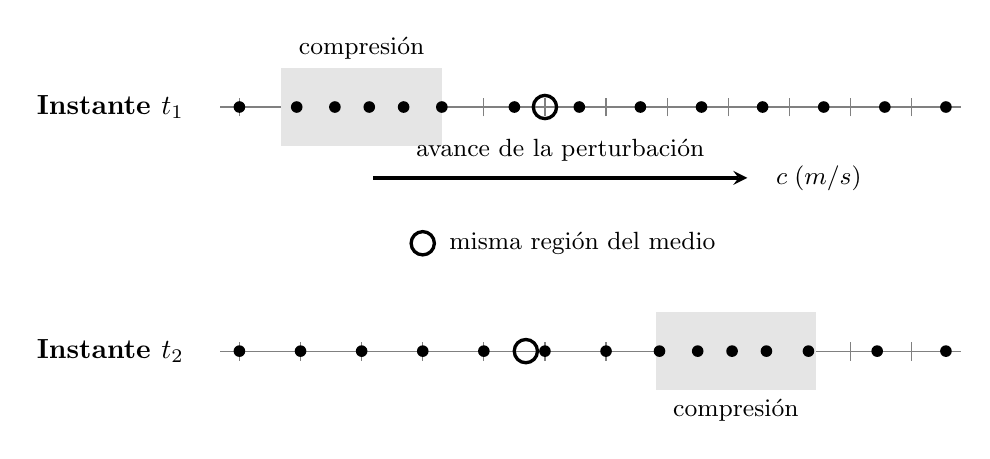
\begin{tikzpicture}[font=\small,>=stealth,x=0.97cm,y=1cm]
    \node[anchor=east,font=\bfseries] at (1.2,1.55) {Instante \(t_1\)};
    \node[anchor=east,font=\bfseries] at (1.2,-1.55) {Instante \(t_2\)};

    % Posiciones de equilibrio.
    \foreach \y in {1.55,-1.55}{
        \draw[gray] (1.55,\y) -- (11.25,\y);
        \foreach \x in {1.8,2.6,...,11.0}{
            \draw[gray] (\x,\y-0.12) -- (\x,\y+0.12);
        }
    }

    % Regiones comprimidas en dos posiciones diferentes.
    \fill[black!10] (2.35,1.05) rectangle (4.45,2.05);
    \fill[black!10] (7.25,-2.05) rectangle (9.35,-1.05);
    \node at (3.40,2.30) {compresión};
    \node at (8.30,-2.30) {compresión};

    % Partículas en t1.
    \foreach \x in {1.8,2.55,3.05,3.50,3.95,4.45,5.40,6.25,7.05,7.85,8.65,9.45,10.25,11.05}{
        \fill (\x,1.55) circle (2.1pt);
    }
    % Partículas en t2.
    \foreach \x in {1.8,2.60,3.40,4.20,5.00,5.80,6.60,7.30,7.80,8.25,8.70,9.25,10.15,11.05}{
        \fill (\x,-1.55) circle (2.1pt);
    }

    % Misma región del medio, marcada en ambos instantes.
    \draw[very thick] (5.80,1.55) circle (4.2pt);
    \draw[very thick] (5.55,-1.55) circle (4.2pt);
    \draw[very thick] (4.20,-0.18) circle (4.2pt);
    \node[anchor=west,align=left] at (4.42,-0.18)
        {misma región del medio};

    % Avance de la perturbación.
    \draw[->,very thick] (3.55,0.65) -- (8.45,0.65)
        node[midway,above=2pt] {avance de la perturbación};
    \node[anchor=west,align=left] at (8.70,0.65)
        {\(c\;(\text{m}/\text{s})\)};
\end{tikzpicture}
